\section{Data}
\label{sec:data}

We use Python \citep{python3} to analyze S\&P500 price data from Yahoo Finance \citep{yahoo_finance_gspc} and the Fama-French 3-factor data library \citep{french_website}.
Yahoo finance provides daily price data of the S\&P500 which we resample to monthly returns for the period 1950 - 2024. We get monthly log returns by taking the
difference of the log of the adjusted close price of the S\&P500 for each month.

\subsection{Cumulative Log Returns}
The unbiasedness regression require windows of cumulative returns. For any month t, we get every forward month's returns up to T months.
By taking expanding window sums of the columns of log returns, we get a cumulative log returns matrix.
% An illustrative example can be found in Table~\ref{tab:sp500_cumulative_returns}.

% \begin{table}[h!]
%     \centering
%     \renewcommand{\arraystretch}{1.5} % Adjust row height
%     \begin{tabular}{|p{3cm}|p{2.5cm}|p{2.5cm}|p{2.5cm}|p{2.5cm}|p{2.5cm}|}
%         \hline
%         \textbf{Date} & \shortstack{\textbf{Cumulative}\\\textbf{Returns t=0}} & \shortstack{\textbf{Cumulative}\\\textbf{Returns t=1}} & \shortstack{\textbf{Cumulative}\\\textbf{Returns t=2}} & \shortstack{\textbf{Cumulative}\\\textbf{Returns t=3}} & \shortstack{\textbf{Cumulative}\\\textbf{Returns t=4}} \\
%         \hline
%         1950-01-01 & 0.01 & 0.03 & 0.06 & 0.10 & 0.15 \\
%         1950-02-01 & 0.02 & 0.05 & 0.09 & 0.14 & 0.20 \\
%         1950-03-01 & 0.03 & 0.07 & 0.12 & 0.18 & 0.25 \\
%         1950-04-01 & 0.04 & 0.09 & 0.15 & 0.22 & 0.30 \\
%         1950-05-01 & 0.05 & 0.11 & 0.18 & 0.26 & 0.35 \\
%         \hline
%     \end{tabular}
%     \caption{Example of the SP500 cumulative returns matrix}
%     \label{tab:sp500_cumulative_returns}
% \end{table}


\subsection{The Value Spread}

The value spread is the ratio of the price-to-book of the portfolio of the portfolio of the most expensive 30\% of stocks to the price-to-book of the portfolio of the cheapest 30\% of stocks, as per \citet{fama_french_1993}.
To construct this measure we use Kenneth French's data library \citep{french_website}. 
Using French’s 3x2 sort on price-to-book and market equity, we get the monthly market value weighted average of the price-to-book of the portfolio of the 30\% most expensive large-cap stocks and the portfolio of the 30\% cheapest large-cap stocks. The value spread is the ratio of these two portfolios.
It represents how much more expensive the expensive stocks are compared to the cheap stocks.
 Figure~\ref{fig:value_spread}.

\begin{figure}[h!]
    \centering
    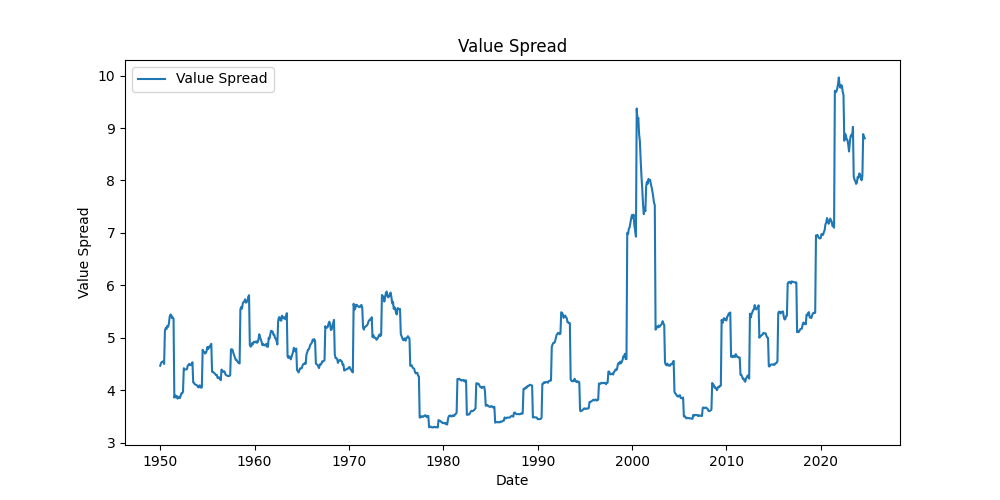
\includegraphics[width=0.8\textwidth]{../figs/Value Spread.png}
    \caption{The value spread timeseries 1950 - 2024}
    \label{fig:value_spread}
\end{figure}
